\section{Я чуть  чуть опаздал}

\subsection{Многообразие с краем}

\paragraph*{Напоминание}

$k$--мерную $r$--гладкую поверхность в $\R^n$ (многообразие без края).

Пусть $\mathcal M \subseteq \R^n, x^0 \in \mathcal M$.

Окрестность $U_M (x^0) = m \cap U(x^0)$, где $U(x^0)$ --- открытое в $\R^n$.

$\exists ~$ открытое $D \subseteq \R^k$, ~$\Phi : D \to U_M(x^0)$, где
$\Phi \in C^k (D)$, регулярно.

\begin{definition}
    Стандартный куб в $\R^k$ --- это $(-1, 1)^k$.
\end{definition}

\begin{definition}
    Стандартный полукуб в $\R^k$ --- это $[-1, 0] \times (-1, 1)^{k -1}$ при $k > 1$ и $(-1, 0]$ или $[0, 1)$ при $k = 1$.
\end{definition}

\begin{center}
    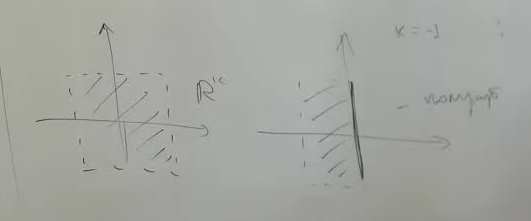
\includegraphics[scale=0.55]{img/simple-squere-and-halfsquere.png}
\end{center}

\begin{definition}
Пусть $\mathcal M \subseteq \R^n$. $\mathcal M$ называется $k$--мерным многообразием с краем, если $\forall x^0 \in \mathcal M \exists $ окрестнось $U_M (x^0)$ и $\Phi ~:~ \Pi_k \to U_M (x^0)$, регулярно и $\in C^k$.

Здесь $\Pi_k$ --- стандартный $k$--мерный куб или стандартный $k$--мерный полукуб.
\end{definition}

$U_M (x^0)$~--- стандартныя окрестнось точки $x^0$  в $\mathcal M$.

$\Phi$~--- локальная параметризация (стандартная).

$\langle U_M(x^0), \Phi\rangle $~--- карта; набор карт~--- атлас.

\begin{example}Очевидные:
    \begin{enumerate}
        \item $(-1, 1)^k$~--- $k$--мерное многообразие (без края).
        \item $(-1, 0] \times (-1, 1)^{k-1}$~--- $k$--мерное многообразие с краем.
        \item $\mathbb{M}_{k, n}^{(r)}$~--- набор $k$--мерных многообразий с краем в $\R^n$ гладкости $r$.
    \end{enumerate}
\end{example}

\begin{center}
    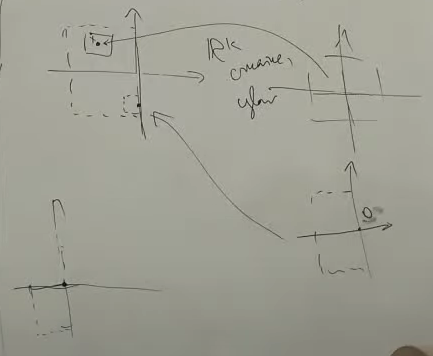
\includegraphics[scale=0.5]{img/k-dimensional-variety-ex1.png}
\end{center}

\begin{example} Чуть менее очевидныей пример.

    $\R^n \in \mathbb{M}_{n,n}^{(\infty)}$~--- многообразие с краем (край пустой).

    \[ \Phi(x_1, \dots, x_n) = \left( \tg \left(x_1 \cdot \dfrac{\pi}{2}\right), \tg \left(x_2 \cdot \dfrac{\pi}{2}\right) \right), \dots, \tg \left(x_n \cdot \dfrac{\pi}{2}\right), ~~~ |x_i| < 1.\]
\end{example}

\begin{definition}
    Пусть $\mathcal M \in \mathbb{M}_{k,n}^{(r)}$.  $x^0 \in \mathcal M$ называется внутренней (относительно многообразия), если $\exists $ стандартная локальная параметризация $\Phi ~:~ \Pi \to U_M(x^0)$, такая, что $\Pi$~--- куб.
\end{definition}

Если точка $x^0$ не является внутренней, то она называется крайней (точкой края).

$\partial \mathcal M = $ множество крайних точек $\mathcal M$ (край $\mathcal M$).

\begin{note}
    Если $\exists$ стандартная параметризация $\Phi ~:~ \Pi \to U_M (x^0)$, такая что $\Pi$~--- полукуб, то $\forall $ стандатной параметризации $\psi ~:~ \tl \Pi \to \tl U_M (x^0)$, $\tl \Pi$~--- полукуб.
\end{note}

\begin{center}
    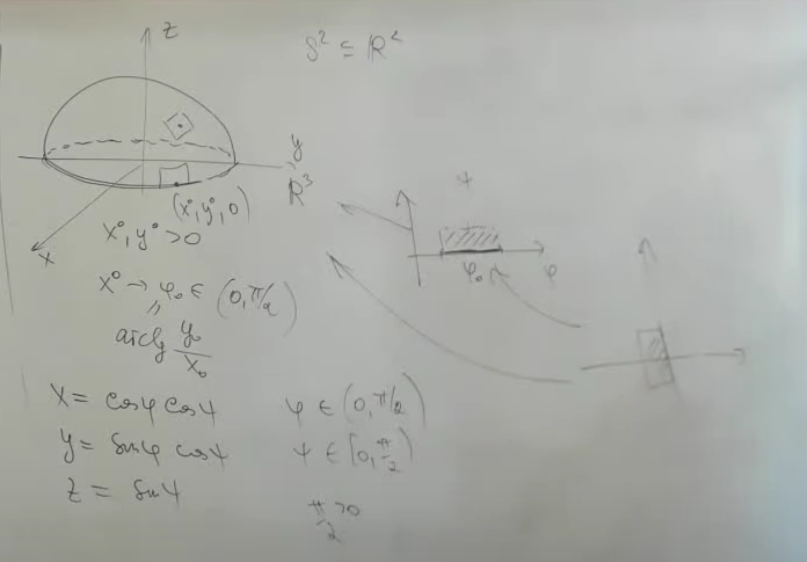
\includegraphics[scale=0.4]{img/halfsphere-to-extreme-points.png}
\end{center}

\begin{note}
    $\mathrm{Fz} \mathcal M \neq \partial \mathcal M$. То есть множество крайних точек не равно множеству граничных точек.
\end{note}

\begin{definition}
    Дискретное множество в $\R^n$ -- множество без предельных точек в $\R^n$

    Само множество не более, чем счётно. В любом шаре $\R^n$ лишь конечное множество точек.

    Дискретное множество в $\R^n$ -- многообразие размерности $0$ в $\R^n$ -- $\mathbb M_{0, n}$
\end{definition}

\begin{example}
    [Конус]

    \[
    ax^2 + by^2 = z^2
    .\]

    В нуле ранг нарушается. Весь конус целиком не многообразие.
\end{example}
% строчк

$\sqsupset  \left( U(x_0), \Phi \right) , \left( \tl U(x_0), \Psi  \right) $ -- две карты для $M in \mathbb M_{k, n}^{(r)},k\in \N $

$V = U(x_0) \cap \tl U(x_0)$

$\Phi^{-1}(C) = W\quad \Psi^{-1}(V) = \tl W$

$\Theta = \Psi^{-1} \circ \Phi\qquad \Theta: W \to \tl W$ -- отображение перехода.

\begin{statement}
    В условия определения отображения перехода оно есть диффеоморфизм из $W$ в $\tl W$.
\end{statement}

\begin{example} Параметризация поверхности сферы через полярные координаты.
    \[ \Phi: (\phi, \psi) \to \begin{bmatrix} \cos\varphi\cos\psi \\ \sin\varphi\cos\psi \\ \sin\psi \end{bmatrix},
    \Psi: (x,y) \to \begin{bmatrix} x \\ y \\ \sqrt{1 - x^2 - y^2}  \end{bmatrix}.\]

    \begin{center}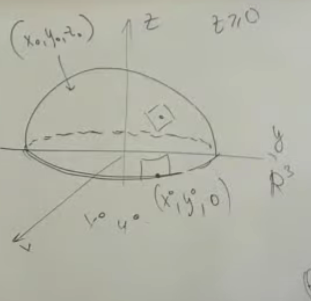
\includegraphics[width=0.25\textwidth]{img/parmetrization-surface-of-sphere.png}
    \end{center}

    \[ \theta: (\varphi, \psi) \to (x,y),~~~
    \theta(\varphi, \psi) = \begin{bmatrix} \cos\varphi\cos\psi \\ \sin\varphi\cos\psi \end{bmatrix},~~~
    \p \theta = \begin{bmatrix}
        -\sin\varphi\cos\psi & -\cos\varphi\sin\psi \\
        \cos\varphi\cos\psi & -\sin\varphi\sin\psi\\
    \end{bmatrix}. \]

    $\det \p \theta = \cos\pi\sin\psi$

    $\pi_{x_1, \ldots, x_k}\Psi : \Pi\in \R^n \to \R^k$ -- локально диффеоморфизм

    $(g = \pi \circ \psi)^{-1}: (x_1, \ldots, x_k) \to (v_1, \ldots, v_k)\qquad x_{k+1}, \ldots, x_n$ -- функции от первых координат

    $\Theta = g \circ \pi_{x_1, \ldots, x_k}\Phi$. Аналогично устроено обратное отображение, значит определители обоих не могут обращаться в ноль.
\end{example}

\begin{corollary}
    Инвариантность типа множества (куб или полукуб) от выбора станратной параметриазации вытекает из последнего утверждения,
\end{corollary}

\begin{corollary}
    $\forall \mathcal M \in \mathbb M_{k,n}^{(r)}\quad \forall x^0\in \mathcal M$ лькально некоторые $n-k$ координат точки выражаются как функции от остальных координат.
\end{corollary}

\begin{note}
  Касательное пространство -- пространство касательных векторов (векторов принадлежащих какой-то кривой на поверхности).

    $\Tp \mathcal M = d_{\Phi^1(p)}\Phi(\R^k)$
\end{note}

\begin{definition}
    $\sqsupset \mathcal M \in \mathbb M_{k, n}^{(1)}\quad x^0\in \mathcal M\quad (U(x_0), \Phi)$ -- карта

    $T_{x_0}\mathcal M = d_0\Phi(\R^k)$
\end{definition}

\begin{note}
    Определение $T_{x^0}\mathcal M$ не зависит от параметризации.
    \[
    d_0\Phi(\R^k) = d_0(\Psi_0\theta)(\R^k) = f_{\theta(0)}\Psi(d_0\theta (\R^k))  = d_{\theta(0) = 0}\Psi(\R^k)
    .\]

    $d_0\theta$ -- изоморфизм, т.к. $\theta$ -- диффеоморфизм.
\end{note}

\begin{note}
    $N \in \R, N$ -- нормальный вектор к $\mathcal M$  в точке $x^0$, если $N \perp T_{x^0}\mathcal M$. (Иногда требуют длину 1, но часто нет)
\end{note}
\begin{note}
    Если $M\in \mathbb M_{k,n}^r$ в окрестности $x^0$ задаётся системой $\begin{cases}
        F_1(x) = 0\\
        \ldots\\
        F_{n-k}(x) = 0\\
    \end{cases}$

    $\nabla F_1, \ldots, \nabla F_{n-k}$ -- базис $(T_{x^0} \mathcal M)^{\perp}$

\end{note}

\begin{note}
    Если $\mathcal M\in M_{n-1,n}^{(1)}\quad N \perp T_{x^0}\mathcal M\quad N = \left|
        \begin{matrix}
            e_1& e_2& \ldots& e_n\\
            && \frac{\partial \Phi}{\partial u_1}(0)&\\
            && \vdots&\\
            && \frac{\partial \Phi}{\partial u_n}(0)&\\
        \end{matrix}
    \right| $

    $(U(x_0), \Phi)$ -- карта

    $\iff N \perp \frac{\partial \Phi}{\partial u_j}(0)\quad \forall j = 1, \ldots, n-1$

    $\left<N, \frac{\partial \Phi}{\partial u_j}(0) \right> = \left|
        \begin{matrix}
            && \frac{\partial \Phi}{\partial u_j}(0)&\\
            && \frac{\partial \Phi}{\partial u_1}(0)&\\
            && \vdots&\\
            && \frac{\partial \Phi}{\partial u_n}(0)&\\
        \end{matrix}
    \right| = 0 $, т.к. совпадают две строки.

    Частный случай. Пусть $n = 3$, $k = 2$. $\mathcal M$~--- график $z = g(x, y)$, заданный на открытом множестве $D \subseteq \R^2$, $g \in C^1$.

    \[ \Phi :(x, y) \to (x, y, z) = (x, y, g(x, y)),~~~
     \p \Phi = \begin{pmatrix}
        1 & 0 \\ 0 & 1 \\ \p g_x & \p g_y
    \end{pmatrix}\]

    Таким образом, $\mathcal{M}$~--- двумерное многообразе хотя бы класса $C^{(1)}$, то есть $\mathcal M \in \mathbb M_{2, 3}^{(1)}$.

    $N$~--- нормаль к $\mathcal{M}$, ~$N = \begin{bmatrix}
        \vec{i}& \vec{j} & \vec{k} \\ 1 & 0 & \p g_x \\ 0 & 1 & \p g_y
    \end{bmatrix} = \left( -\p g_x , -p g_y, 1 \right)$~--- направлена вверх.
\end{note}

\begin{definition}
    $\sqsupset (U(x^0), \Phi), (\tl U(x^0), \Psi)$ -- две карты

    $x_0\in \mathcal M\quad \mathcal M\in \mathbb M_{k, n}^{(r)}$

    Скажем, что $\Phi$ и $\Psi$ согласованы, если $\det \Theta >0$, где $\theta = \Psi^{-1}\circ\Phi$ -- отображение перехода.
\end{definition}

\begin{note}
    Отношение согласованности является отношение эквивалентности.
    % Отображение перехода образует отношение эквивалентности.
\end{note}

\begin{definition}
    $I(x^0)$ называется ориентированной, если зафиксирован один из классов экивалентности по отношению согласованности.
\end{definition}

\begin{note}
    $\sqsupset U(x^0) \cap U(x^1) \neq 0$. $U(x^0)$ И $U(x^1)$  согласованы, если $\Phi\in U_+(x^0), \Psi\in U_+(x^1)$, где $U_+$ -- зафиксирванный класс.
    $ \implies \det(\Psi^{-1}\circ\Phi) >0$

    Если $U(x^0) \cap U(x^1) = \O $, то их ориентации согласованы.

    Атлас $A = \{(U, \Phi)\}$ многообразия $\mathcal M$ называется ориентированным, если ориентации любых двух $U, V\in A$ согласованы.

    Многообразие с краем называется ориентиркемым, если $\exists $ ориентированный атлас.
\end{note}

\begin{definition}
    Пусть $\Gamma = \mathcal{M} \in \mathbb{M}_{1, n}^{(1)}$, ~ $\tau ~:~ \mathcal M \to \R^n$ и $\forall x^0 \in \mathcal{M}~:~ \tau (x^0) \in T_{x^0} \circ \mathcal M$, ~$\tau$~--- непрерывное, $\|\tau\| \equiv 1$.

    Тогда $\tau$ называется направлением на $\mathcal M$.
\end{definition}


\begin{statement}
    $\forall $ связное $1$--менрное, $1$--глакое многообразе с краем имеет ровно два направления.

    $ \tau (x) =  \pm \dfrac{\p \gamma}{\| \p \gamma \|} ~~(\gamma ^{-1} (x))$, где $\gamma$~--- параметризация из выбранного класса эквивалентности (из ориентации окрестности $\mathcal{M}$).
\end{statement}

\begin{definition}
    $k = n-1\quad n\in \N , n\geqslant 2\quad \mathcal M \in \mathbb M_{n-1, n}^{(\perp)}$

    $n(x) : \mathcal M \to \R^n$ называется стороной, если:
    \begin{enumerate}
        \item $n(x)\in C(M)$
        \item $\forall x\in \mathcal M\quad n(x)\perp T_x \mathcal M$
        \item $\|n(x)\| = 1$
    \end{enumerate}
\end{definition}

\begin{note}
    Сторон чётное число.
\end{note}

\begin{note}
    Не у всех поверхностей есть сторона. Лента Мёбиуса, бутылка Клейна, \ldots

    \begin{center}
        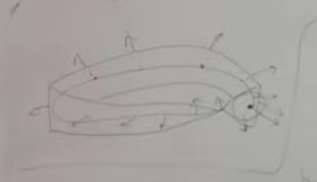
\includegraphics[scale=0.5]{img/moebius-tape.png}
    \end{center}
\end{note}

\begin{statement}
    Для $k = n-1$ ориентируемость многообразия с краем $\mathcal M \in (\mathbb M_{n-1, n}^1)$ равносильно существоавнию стороны.
\end{statement}

\begin{theorem}
    Пусть $\mathcal M\in \mathbb M^{(1)}_{k, n}\quad K\leqslant n, k, n\in \N $

    Тогда:
    \begin{enumerate}
        \item $\partial \mathcal {M} \in \mathbb{M}_{k-1 ,n}^{(1)}$; $\partial \left(\partial \mathcal{M}\right) = \varnothing $
        \item Если $\mathcal M$ -- ориентированно то $\partial \mathcal M$ ориентируем.
    \end{enumerate}
\end{theorem}
\begin{proof}
    $\partial \mathcal M$ -- многообразие без края.
\end{proof}

\begin{center}
    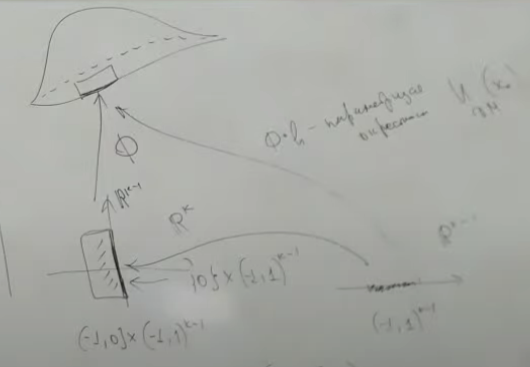
\includegraphics[scale=0.4]{img/extreme-points-of-extreme-points-ex1}
\end{center}

%%%
\begin{note}[Воспоминания]
    Многообразие -- локально гомеоморфно кубу.

    С краем -- есть точки геомеоморфные половине куба.

    Пусть у нас есть две параметризации окрестности: $\Phi, \Psi. \Phi = \Psi \circ \Theta\qquad \Phi \sim \Psi \iff \det \p \Theta > 0$

    Класс эквивалентности $\left[ \Phi \right] $ -- ориентация окрестности

    $U, V$ -- окрестности в  $M$. Они согласованы если:
     \begin{itemize}
        \item они не перескекаются
        \item они пересекаются и $\det \p \theta > 0$, где $\theta$ -- отображение перехода от  $\Phi$ к  $\Psi$, где  $\Phi$ -- из ориентации  $U$,  $\Psi$ -- из ориентации  $V$ и  $\Phi(\Pi) \cap \Psi(\Pi) \neq \O $        
    \end{itemize}
\end{note}

\begin{example}
    $S_1 = S \cap \left\{ z>0 \right\} \quad S_2 = S \cap  \left\{ x>0 \right\} $

    $\theta: (x,y) \to (y, \sqrt{1 - x^2-y^2} $ 

    $\p \theta = \begin{bmatrix} 0&1\\ -\frac{x}{\sqrt{1-x^2-y^2} }& -\frac{y}{\sqrt{1 - x^2-y^2} } \end{bmatrix} $

    $\p \det = \frac{x}{\sqrt{1 - x^2-y^2} }>0$ на области определения ($\Phi^{-1}(S_1\cap S_2)$ )

    $S_3 = S \cap \left\{ z<0 \right\} \quad $

    $\tl \theta(x,y) = (y, -\sqrt{1-x^2-y^2} $ 

    И здесь уже всё плохо с определиителем.
\end{example}

\begin{statement}
    $\sqsupset \gamma: \left<a,b \right>\subseteq \R \to \R^n $, регулярно ($\iff  \p \gamma(t) \neq 0\quad \forall t\in \left<a,b \right>$). $\gamma$ -- простой путь (без самопересечений, инъективность)

    $\Gamma = \gamma\left( \left<a,b \right> \right) $ -- Одномерное многообразие.

    Край не пуст, если $\left\{ a,b \right\} \cap \left<a,b \right>\neq \O $

    Направление -- непрерывное отображение $\tau:\Gamma \to \R^n$:
    \begin{enumerate}
        \item непрерывно $\tau\in C(\Gamma)$
        \item  $\tau(x) \in T_x\Gamma \forall x\in \Gamma$
        \item $\|\tau(x)\| = 1 \forall x\in \Gamma$
    \end{enumerate}

    Для любой гладкой кривой $\Gamma$ (из определения выше) существует ровно два направления на этой кривой, и любая такая  $\Gamma$ ориентируема
\end{statement}
\begin{proof}
    Ориентация порождается сужениями одного и того же отображения $\lambda$ на различные кубы и полукубы.

    \[
        \tau_\gamma = \frac{\p \gamma}{\|\p \gamma\|}\left( \gamma^{-1}(x) \right) 
    .\] 
    $\tau(x)$ -- ещё одно направление

    $t\in \left( a,b \right) \quad h(t) = \left<\tau_\gamma\left( \gamma(t) \right) , \tau(\gamma(t)) \right> = \pm \|\tau_\gamma\left( \gamma(t) \right) \| \|\tau\left( \gamma(t) \right) \| = \pm 1 $

    $h: \left<a,b \right> \to \left\{ -1,+1 \right\} $ -- непрерывно, но $h(\left<a,b \right>)$ должно быть промежутком:
    \begin{enumerate}
        \item $h\left( \left<a,b \right> \right)  = \left\{ 1 \right\} \implies \tau = \tau_\gamma$
        \item $h\left( \left<a,b \right> \right)  = \left\{ -1 \right\} \implies \tau = -\tau_\gamma$
    \end{enumerate}
\end{proof}

\begin{statement}
    $k = n-1\geqslant 2, n\in \N$

    Сторона на многообразии $M\in \mathds M_{n-1, n}^1$ -- отображение  $N: M \to \R^n$:
    \begin{enumerate}
        \item $n\in C\left( M \right) $
        \item $N(x) \perp T_x M$ 
        \item $\|N\| = 1$
    \end{enumerate}

    Если $M\in \mathds M_{n-1, n}^1$. Тогда $M$ двусторонняя $\iff M$ ориентируема. Если $M$ двустороняя, то любая сторона представима в виде:
    \[
        N = \pm\frac{N_{\Phi}}{\|N_\Phi\|}\left( \varphi^{-1}(x) \right) 
    .\] 
    $\Phi$ -- параметризация окрестности точки  $x$ Из выбранной ориентации  

    $N_\Phi = 
    \begin{vmatrix}
        \vec e_1 & \ldots & \vec e_n\\
        \ldots & \p \Phi_{u_1} & \ldots\\
        \ldots& \vdots & \ldots\\
        \ldots & \p \Phi_{u_{n-1}}& \ldots
    \end{vmatrix}$

    $\|N_{\Phi}\| \neq 0$

    $\Phi \sim \tl \Phi$


    
\end{statement}
